\pagestyle{empty}
\centering
\fontsize{2cm}{2cm}\selectfont{Module Design Document} \\
\vspace{2mm}
\fontsize{1cm}{1cm}\selectfont Audio digital signal processor \\
\vspace{2mm}
\large BeCreative Minor\\
\normalsize
\vspace{4cm}
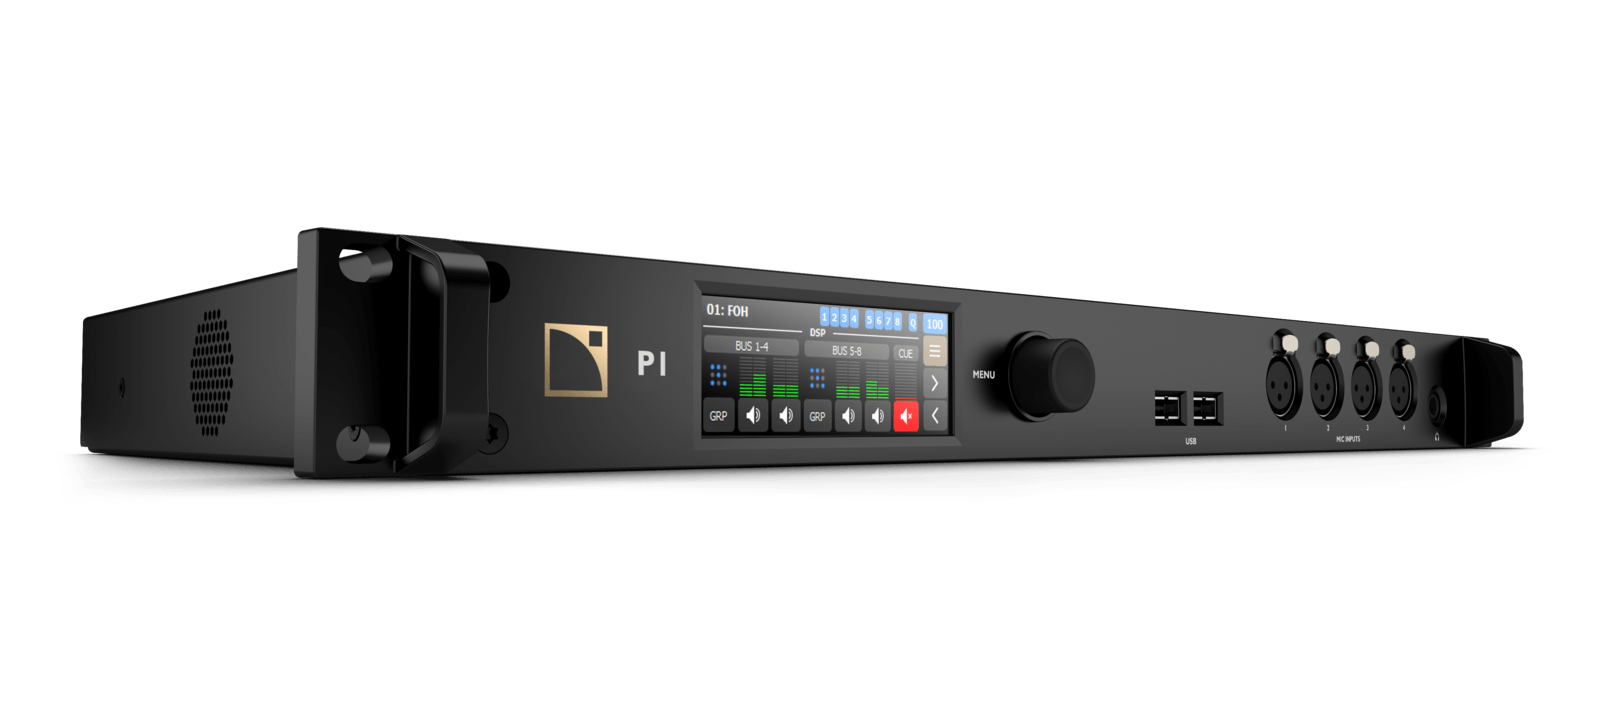
\includegraphics[width=\linewidth]{3DR_P1_Perspective.png}\\
\vfill
\normalsize Busse Lommers \\
Robin van den Dungen \\
Mahmud Gürler \\
Silas Kamphuis \\
Hein Verhallen \\
Youri Tils \\
Fontys Hogescholen, De Rondom 1, 5612 AP Eindhoven \\
\today

\begin{justify}

%\chapter*{Summary}

\newpage
\tableofcontents
\thispagestyle{empty}

\listoffigures
\thispagestyle{empty}


\listoftables
\thispagestyle{empty}

\newpage
\pagestyle{plain}
\setcounter{page}{1}

\chapter*{Abbreviation List}

\begin{table}[!h]
	\centering
\begin{tabular}{|c|c|}
	\hline
\textbf{Abbreviation} & \textbf{Explanation}        \\ \hline
DSP 					& Digital Signal Processor    \\ \hline
ADC 					& Analog-to-Digital Converter \\ \hline
DAC 					& Digital-to-Analog Converter \\ \hline
RAM 					& Random access memory	    \\ \hline
SINAD 				& Signal to noise and distortion \\ \hline
TRS 					& Tip ring sleeve connector (jack) \\ \hline
FPGA 					& Field programmable gate array \\ \hline
CH 						& Channel					\\ \hline
FFT 					& Fast Fourier Transform	\\ \hline
BPF 					& Band-Pass Filter			\\ \hline
SEPIC         & Single-ended primary-inductor converter			\\ \hline

\end{tabular}
\caption{List of commonly used Abbreviations}
\label{Abbreviation list}
\end{table}